\chapter{Risultati ottenuti}
\label{risultati}

\section{Risultati ottenuti sul dataset GPD}
\subsection{Feature hand-crafted}

Per prima cosa sono stati analizzati i risultati ottenuti con le feature hand-crafted, ovvero le più semplici, i quali sono riportati in Tabella \ref{tabella_handcrafted}.

\begin{table}[H]
\resizebox{\columnwidth}{!}{
\centering
\begin{tabular}{| c | c | c | c |}
\hline
Feature & Classificatore & Training Set & Test Set\\ [0.5ex]
\hline
LBP & SVM & 0.7276 & 0.6987 \\
CEDD & SVM & 0.6788 & 0.6529 \\
QHist & SVM & 0.6931 & 0.6904 \\
LBP, CEDD, QHist & SVM & 0.6766 & 0.6667 \\
Media H, Media S, Intensità & SVM & 0.5813 & 0.6075 \\
Pleasure, Arousal, Dominance & SVM & 0.5688 & 0.5850 \\
Media H, Media S, LBP & SVM & 0.7357 & 0.7446 \\
Media H, Media S, CEDD & SVM & 0.6772 & 0.6854 \\
Pleasure, Arousal, Dominance, LBP & SVM & 0.7277 & 0.7383 \\
Pleasure, Arousal, Dominance, CEDD & SVM & 0.6821 & 0.6867 \\
\hline
\end{tabular}}
\caption{Livelli di accuratezza ottenuti sul training set e sul test set utilizzando diverse combinazioni di feature e il classificatore SVM}
\label{tabella_handcrafted}
\end{table}

In questo caso sono state usate principalmente feature legate al colore e alla texture e il miglior risultato sul test set è stato ottenuto combinando la media di canali H e S insieme a LBP, quindi unendo descrittori legati al colore e alla texture. Inoltre in tabella sono stati riportati i risultati su test set e su training set, i quali sono stati divisi come illustrato nel Capitolo~\ref{GPD}, per poter fare un immediato confronto con i risultati ottenuti nel lavoro originale \cite{sheng2021learning}, i quali sono stati riportati in Tabella \ref{tabella_GPD}. 

\subsection{Feature estratte da una rete neurale}

Di seguito, in Tabella \ref{tabella_estrazione}, sono riportati i risultati ottenuti con feature estratte da due layer differenti di una rete ResNet-18 e, in particolare, non c'è una grande differenza di accuratezza estraendo le feature da un layer che si trova più in profondità all'interno della rete come il layer pool5 rispetto a uno che si trova meno in profondità come il layer res3b\_relu, anzi l'accuratezza è leggermente più elevata nel secondo caso.

Di seguito, così come negli studi successivi, verranno riportati i livelli di accuratezza ottenuti sul test set e sul validation set come spiegato precedentemente in Sezione~\ref{divisione} del Capitolo~\ref{metodologie} al fine di utilizzare dei dataset che avessero una numerosità equa di immagini in ognuna delle due classi.

\begin{table}[H]
\centering
\begin{tabular}{| c | c | c | c | c |}
\hline
Rete & Classificatore & Layer & Test Set & Validation Set\\ [0.5ex]
\hline
ResNet-18 & SVM & pool5 & 0.8350 & 0.8452 \\
ResNet-18 & SVM & res3b\_relu & 0.8391 & 0.8478 \\
\hline
\end{tabular}
\caption{Livelli di accuratezza ottenuti sul validation set e sul test set utilizzando il classificatore SVM con delle feature estratte da due diversi layer della rete ResNet-18. Nel primo caso le feature sono state estratte dal layer pool5, il quale si trova alla fine della rete, mentre nel secondo caso dal layer res3b\_relu, il quale si trova a metà della rete}
\label{tabella_estrazione}
\end{table}

\subsection{Uso delle reti neurali per l'intera classificazione}

Quando ci si affida completamente all'uso di una rete neurale è necessario differenziare quando si utilizzi la tecnica dell'Early Stopping rispetto a quando non la si utilizzi, ciò porta nella maggior parte dei casi a uno spreco di tempo e risorse poiché vengono eseguite tutte le epoche del riaddestramento della rete anche se, come già anticipato nel Capitolo~\ref{metodologie}, non è detto che l'uso del Fine Tuning combinato con l'Early Stopping diminuisca il numero di epoche effettivamente svolte in quanto ciò dipende da come vengono impostati i vari parametri e da come cresce l'accuratezza durante l'esecuzione.

I risultati ottenuti senza stop anticipato sono riportati in Tabella \ref{tabella_rete1}, mentre quelli relativi all'esecuzione con Early Stopping sono riportati in Tabella \ref{tabella_rete2}.

\begin{table}[H]
\resizebox{\columnwidth}{!}{
\centering
\begin{tabular}{| c | c | c | c | c | c |}
\hline
Rete & Test Set & Validation Set & Initial Learn Rate &	Epochs & Batch Size \\  [0.5ex]
\hline
ResNet-18 & 0.8882 & 0.89 & 0.0003 & 6 & 10	\\
ResNet-18 & 0.8996 & 0.8905 & 0.0005 & 6 & 10	\\
ResNet-18 & 0.8731 & 0.8849 & 0.00003 & 6 & 10	\\
ResNet-18 & 0.8520 & 0.8493 & 0.00001 & 6 & 10	\\
ResNet-18 & 0.8744 & 0.8829 & 0.0003 & 8 & 10	\\
\hline
\end{tabular}}
\caption{Livelli di accuratezza ottenuti sul validation set e sul test set utilizzando una procedura di Fine Tuning su una rete ResNet-18. Sono stati riportati anche i parametri utilizzati per inizializzare il numero di epoche, la dimensione del batch e il tasso di apprendimento iniziale della rete} 
\label{tabella_rete1}
\end{table}


\begin{table}[H] 
\resizebox{\columnwidth}{!}{
\centering
\begin{tabular}{| c | c | c | c | c | c | c |}
\hline
Rete & Test Set & Validation Set & Initial Learn Rate &	Epochs & Batch Size & Early Stopping \\  [0.5ex]
\hline
ResNet-18 & 0.9051 & 0.9043 & 0.0005 & 6 & 10 & 2 epoche \\	
ResNet-18 & 0.9015 & 0.8946 & 0.0003 & 6 & 10 & 2 epoche \\
ResNet-18 & 0.8579 & 0.8569 & 0.00003 & 6 & 10 & 1 epoca \\
ResNet-18 & 0.8437 & 0.8462 & 0.00001 & 6 & 10 & 1 epoca \\
% Fa tutte e 6 le epoche
ResNet-18 & 0.8799 & 0.8997 & 0.0003 & 8 & 10 & 2 epoche \\
\hline
\end{tabular}}
\caption{Livelli di accuratezza ottenuti sul validation set e sul test set utilizzando una procedura di Fine Tuning su una rete ResNet-18 con Early Stopping dopo una o due epoche, a seconda di quale  valore portasse a un maggior risparmio di tempo, anche se nel caso di stop anticipato dopo una sola epoca con Initial Learn Rate pari a 0.00001 non c'è stato alcun miglioramento in quanto sono state eseguite comunque tutte le epoche del training. Sono stati riportati anche i parametri utilizzati per inizializzare il numero di epoche, la dimensione del batch e il tasso di apprendimento iniziale della rete} 
\label{tabella_rete2}
\end{table}

\section{Risultati ottenuti sul dataset proposto}

\subsection{Analisi delle groundtruth}

Osservando la distribuzione delle groundtruth delle immagini del dataset proposto, la quale è riportata in Sezione~\ref{valutazione} del Capitolo~\ref{metodologie}, si osserva che gli utenti hanno valutato positivamente 73 immagini del dataset e negativamente le restanti 27. Questo risultato è sbilanciato verso la classe positiva, nonostante inizialmente siano state utilizzate 50 immagini professionali e 50 scattate da utenti comuni non professionisti, ciò mostra come la percezione dell'estetica dei cibi, ma anche in qualsiasi altro ambito, non è strettamente legata alla tecnica fotografica utilizzata o alla struttura della fotografia bensì entrano in gioco anche altri fattori soggettivi, tra cui il background culturale, le abitudini alimentari e gli specifici gusti del sottoinsieme di utenti che sono stati chiamati a valutare le immagini del dataset proposto.

\subsection{Uso di una rete neurale adattata}

Come già anticipato nel Capitolo~\ref{metodologie} per valutare l'estetica nel dataset proposto è stata utilizzata principalmente la rete neurale che ha ottenuto i migliori risultati ovvero, come riportato in Tabella \ref{tabella_rete2}, quella che ha un Initial Learn Rate pari a 0.0005 e che utilizza l'Early Stopping dopo due epoche nelle quali l'accuratezza non migliora.

Utilizzando come groundtruth le label ottenute dal questionario che è stato sottoposto a 41 utenti, la cui distribuzione è stata analizzata precedentemente, e la rete precedentemente citata è stata ottenuta una accuratezza del 72\%.

In questa fase è stata molto significativa l'analisi degli errori compiuti dalla rete e la successiva analisi delle immagini generate con la tecnica Grad-CAM \cite{selvaraju2017grad}, in particolare si evince che la rete ha classificato 17 immagini come falsi negativi, ovvero è stata predetta la label negativa mentre la groundtruth era positiva, e 11 falsi positivi, ovvero è stata predetta la label positiva mentre la groundtruth era negativa. 

Di seguito, in Figura \ref{gradcam_neg} e in Figura \ref{gradcam_pos}, sono riportate alcune delle immagini del dataset proposto a cui è stata applicata la tecnica Grad-CAM e dove la rete non ha compiuto errori di classificazione.

\begin{figure}[H]
\centering
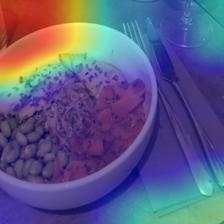
\includegraphics[height=45mm]{images/gradcam1.jpg}
\quad
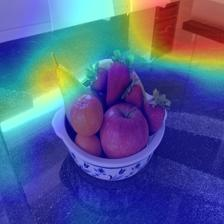
\includegraphics[height=45mm]{images/gradcam23.jpg}
\quad
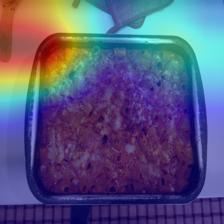
\includegraphics[height=45mm]{images/gradcam14.jpg}
\quad
\caption{Esempi di immagini a cui è stata applicata la tecnica Grad-CAM dove la rete ha predetto correttamente una label negativa}
\label{gradcam_neg}
\end{figure}

\begin{figure}[H]
\centering
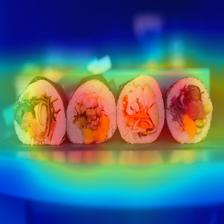
\includegraphics[height=45mm]{images/gradcam53.jpg}
\quad
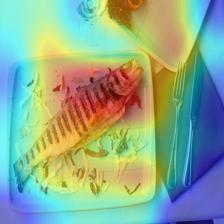
\includegraphics[height=45mm]{images/gradcam85.jpg}
\quad
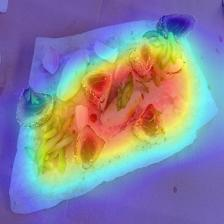
\includegraphics[height=45mm]{images/gradcam28.jpg}
\quad
\caption{Esempi di immagini a cui è stata applicata la tecnica Grad-CAM dove la rete ha predetto correttamente una label positiva}
\label{gradcam_pos}
\end{figure}

In Figura \ref{FalseNeg} è riportato un esempio di immagine appartenente ai falsi negativi, mentre in Figura \ref{FalsePos} è invece riportato un esempio di immagine appartenente ai falsi positivi. Entrambe le immagini di esempio sono riportate insieme alle rispettive Grad-CAM al fine di poter mostrare eventuali differenze nella posizione delle aree più significative, in rosso, e di quelle meno significative, in blu, rispetto al cibo. Questa tematica verrà approfondita nella Sezione~\ref{analisiGradCAM} insieme ad altre ipotesi scaturite dall'analisi delle Grad-CAM, le quali hanno portato a investigare la correlazione tra l'indicatore di concentrazione dell'energia e le predizioni della rete.

\begin{figure}[H]
\centering
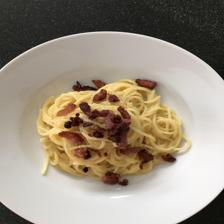
\includegraphics[height=45mm]{images/falseNegImg.jpg}
\quad
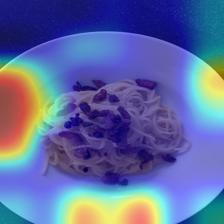
\includegraphics[height=45mm]{images/falseNegCAM.jpg}
\quad
\caption{Esempio di una immagine per la quale la rete ha predetto la label negativa mentre la groundtruth era positiva, per cui essa rientra tra gli errori e in particolare tra i falsi negativi. A destra viene riportata anche la rispettiva Grad-CAM, dalla quale si nota che le aree che la rete ha considerato più significative per la predizione della label non sono quelle del cibo, bensì appartengono al piatto e allo sfondo}
\label{FalseNeg}
\end{figure}

\begin{figure}[H]
\centering
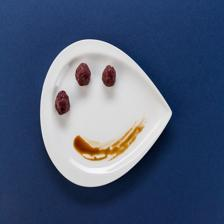
\includegraphics[height=45mm]{images/falsePosImg.jpg}
\quad
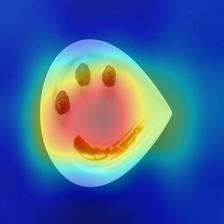
\includegraphics[height=45mm]{images/falsePosCAM.jpg}
\quad
\caption{Esempio di una immagine per la quale la rete ha predetto la label positiva mentre la groundtruth era negativa, per cui essa rientra tra gli errori e in particolare tra i falsi positivi. A destra viene riportata anche la rispettiva Grad-CAM, dalla quale si nota che le aree che la rete ha considerato più significative per la predizione della label sono effettivamente quelle del cibo e non altre parti dell'immagine}
\label{FalsePos}
\end{figure}

\subsection{Analisi delle Grad-CAM}
\label{analisiGradCAM}
Come già evidenziato in precedenza l'analisi delle immagini ricavate con la tecnica Grad-CAM è fondamentale al fine di individuare cosa la rete consideri significativo per l'effettiva predizione della label ed eventualmente per individuare nessi causali tra queste aree, considerate più significative per la predizione, e gli errori compiuti. Infatti osservando le Grad-CAM sembrava che quando l'area più significativa veniva individuata al di fuori del cibo la rete predicesse la label negativa, perciò si è scelto di indagare più a fondo sfruttando l'indicatore di concentrazione dell'energia. 

Per confermare quest'ultima ipotesi è stato costruito un grafico, visibile in Figura \ref{graficoRappPred}, nel quale l'indicatore di concentrazione, riportato sull'asse x e calcolato come espresso in Formula (\ref{indicatore}), viene correlato alle predizioni della rete, riportate sull'asse y. Al fine di rappresentare le label in maniera numerica si è scelto di far corrispondere alla label negativa il valore -1 e alla label positiva il valore 1, in modo tale che la distinzione nel grafico fosse evidente, inoltre si è scelto un grafico di tipo Scatter Plot perché visivamente mostra molto bene la distribuzione dei punti e perché esso dava la possibilità di inserire sugli assi cartesiani due diverse variabili, che in questo caso sono le predizioni e l'indicatore di concentrazione C.

Osservando il grafico è ben visibile che gli elementi della classe positiva sono molto più numerosi di quelli della classe negativa, le immagini sono infatti classificate dalla rete come segue:
% eventualmente togliere \newpage, in questo caso l'ho messo per far si che non si "spezzasse" l'elenco puntato
\newpage
\begin{itemize}
\item \textbf{Classe positiva}: 67 elementi
\item \textbf{Classe negativa}: 33 elementi
\end{itemize}

É molto interessante la distribuzione vera e propria di questi elementi, rappresentati nello Scatter Plot come dei pallini, poiché si nota che al di sopra di un certo valore di soglia, che potrebbe essere individuato attorno al valore 1 sull'asse delle x, è possibile separare le due classi commettendo pochi errori. Questa distribuzione mostra una correlazione tra le variabili inserite sugli assi cartesiani così come era stato ipotizzato, al crescere dell'indicatore di concentrazione dell'energia all'interno dell'area corrispondente al cibo cresce la probabilità che venga predetta la label positiva, in particolare man mano che aumenta la concentrazione si osserva che le predizioni diventano tutte appartenenti alla classe positiva.

\begin{figure}[H]
\centering
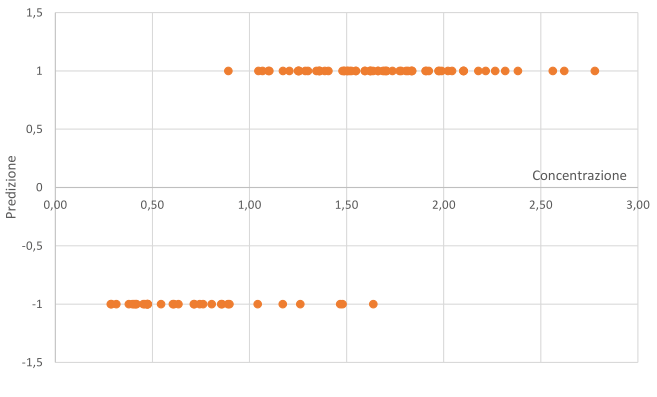
\includegraphics[height=87mm]{images/graficoRappPred.png}
\caption{Grafico che rappresenta sull'asse delle x l'indicatore di concentrazione per ognuna delle immagini del dataset proposto, mentre sull'asse delle y rappresenta le label predette, in particolare il valore -1 indica la label negativa mentre il valore 1 indica la label positiva}
\label{graficoRappPred}
\end{figure}

Questo risultato è davvero significativo poiché conferma l'ipotesi fatta in precedenza, mostrando che quando la Grad-CAM si focalizza correttamente sulla porzione di immagine occupata dal cibo si avrà che la concentrazione di energia in quell'area sarà elevata e, quindi, sarà più probabile che la rete predica una label positiva.

Il risultato va però contestualizzato, in determinati casi entrano in gioco fattori di gusto personale degli utenti e fattori legati alla semantica dell'immagine analizzata che possono essere imprevedibili per la rete neurale in quanto, come già sottolineato, l'estetica è una caratteristica puramente soggettiva e che può variare nel tempo, in quanto un utente potrebbe valutare positivamente un cibo e, in un momento successivo, valutare lo stesso cibo in maniera opposta poiché il suo background culturale e il suo bagaglio di esperienze potrebbero avergli fatto modificare la sua personale concezione di bellezza.





